%!TEX root = index.tex
\chapter{State of the art}
\section{Definitions}

Air Traffic Control service (ATC) can be devided into: area control service (ACC), approach control service (APP) and aerodrome control service (TWR) \cite[Chapter 1]{ICAO2007} The main objective is to prevent collisions between aircraft in air or on land and to expedite the flow of air traffic. \cite[Chapter 2.2]{annex11}
The airspace in which ATC service is provided can be divided into Control area (CTA), Control Zones (CTR) and Controlled aerodromes (TWR). Control area contains airways, terminal control areas and other airspace. It extends upwards from specified altitude. Within CTA, terminal control areas (TMA) are established to help in arrival and departure at some airports.
Control zones are normally situated below CTA and encompass airspace used by flights arriving at and departing from aerodromes.

The controlled airspace can furthermore be classified as Class A-G. \cite[\textcolor{red}{ref na nolana}]{NOLAN}

\textcolor{red}{Pro řízení v terminální oblasti nás zajímají všechny druhy řízení/prostoru, Agentfly má zatím jen ACC v CTA?}

\begin{figure}[h]
    \centering
    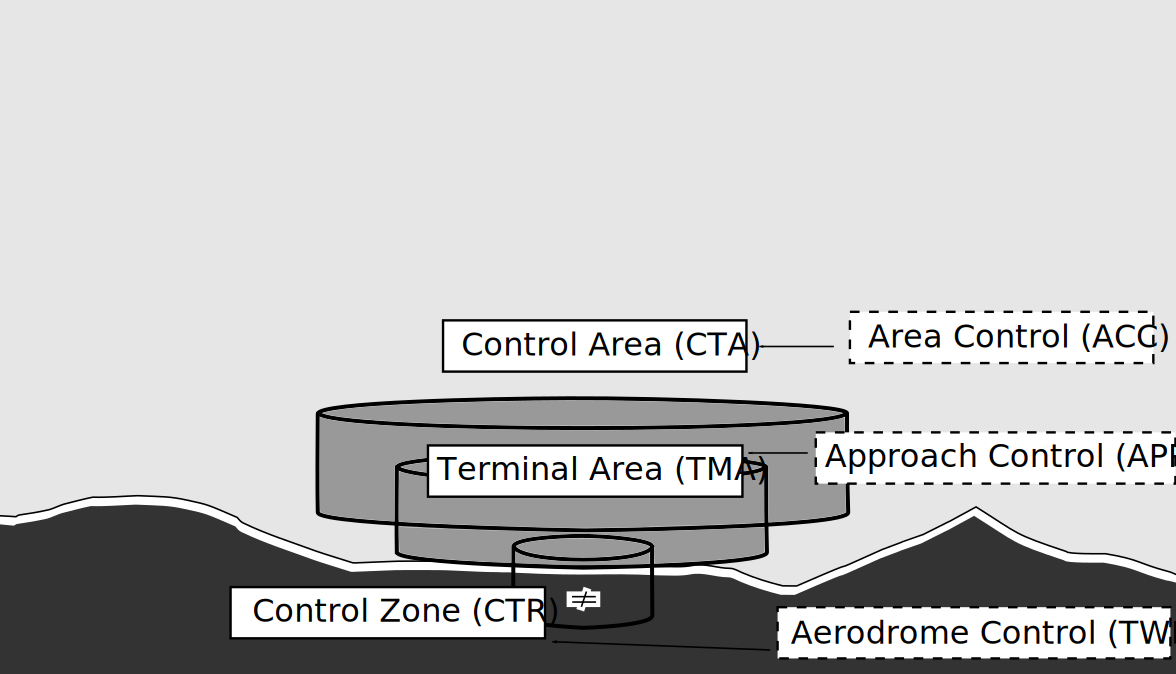
\includegraphics[width=0.8\textwidth]{figures/airspace.png}
    \caption{Airspace - \textcolor{red}{z prezentace 2011 ATM Lesson Plans/ATM 1-1 General Air Traffic Services podle \cite[Chapter 2.5]{annex11} - překreslit!}}
    \label{fig:airspace}
\end{figure}

\begin{figure}[h]
    \centering
    \includegraphics[width=0.8\textwidth]{figures/cta.png}
    \caption{CTA - \textcolor{red}{z prezentace 2011 ATM Lesson Plans/ATM 1-1 General Air Traffic Services podle \cite[Chapter 2.10]{annex11} - překreslit!}}
    \label{fig:airspace}
\end{figure}